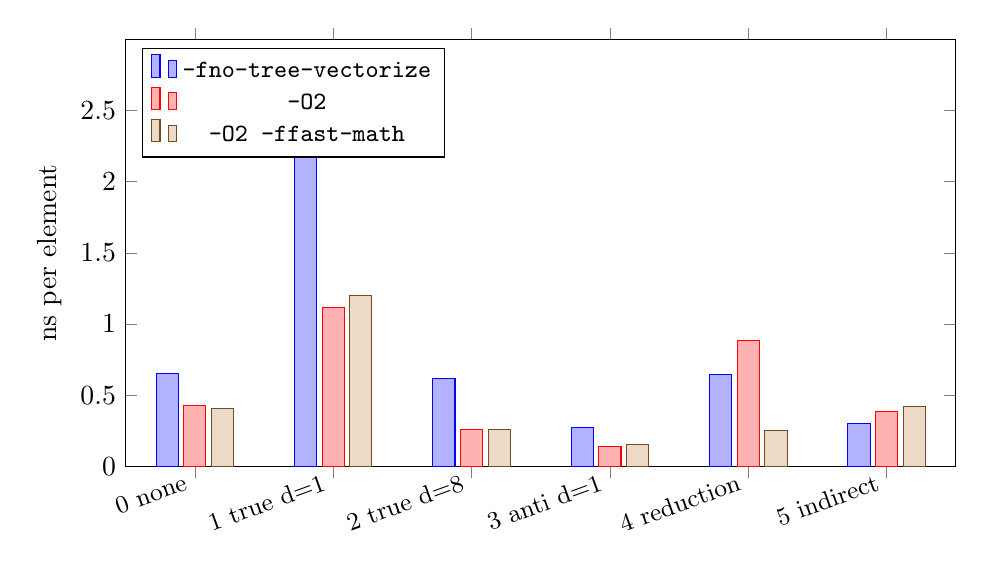
\begin{tikzpicture}
\begin{axis}[ybar, width=\textwidth, height=7cm, bar width=8pt, ymin=0, ylabel={ns per element}, symbolic x coords={0 none,1 true d=1,2 true d=8,3 anti d=1,4 reduction,5 indirect}, xtick=data,
  x tick label style={rotate=20, anchor=east, font=\small}, legend style={font=\small, at={(0.02,0.98)}, anchor=north west}, enlarge x limits=0.1]
\addplot coordinates {(0 none,0.6505) (1 true d=1,2.7235) (2 true d=8,0.6160) (3 anti d=1,0.2749) (4 reduction,0.6476) (5 indirect,0.3035)};
\addlegendentry{\texttt{-fno-tree-vectorize}}
\addplot coordinates {(0 none,0.4307) (1 true d=1,1.1138) (2 true d=8,0.2565) (3 anti d=1,0.1410) (4 reduction,0.8864) (5 indirect,0.3838)};
\addlegendentry{\texttt{-O2}}
\addplot coordinates {(0 none,0.4075) (1 true d=1,1.2010) (2 true d=8,0.2564) (3 anti d=1,0.1557) (4 reduction,0.2491) (5 indirect,0.4192)};
\addlegendentry{\texttt{-O2 -ffast-math}}
\end{axis}
\end{tikzpicture}